% !TeX spellcheck = en_GB

%----------------------------------------------------------------------------------------
%	PACKAGES AND OTHER DOCUMENT CONFIGURATIONS
%----------------------------------------------------------------------------------------

\documentclass[
11pt, % The default document font size, options: 10pt, 11pt, 12pt
oneside, %TODO: % Two side (alternating margins) for binding by default, uncomment to switch to one side
english, % ngerman for German
singlespacing, % Single line spacing, alternatives: onehalfspacing or doublespacing
%draft, % Uncomment to enable draft mode (no pictures, no links, overfull hboxes indicated)
%nolistspacing, % If the document is onehalfspacing or doublespacing, uncomment this to set spacing in lists to single
liststotoc, % Uncomment to add the list of figures/tables/etc to the table of contents
toctotoc, % Uncomment to add the main table of contents to the table of contents
%parskip, % Uncomment to add space between paragraphs
%nohyperref, % Uncomment to not load the hyperref package
headsepline, % Uncomment to get a line under the header
%chapterinoneline, % Uncomment to place the chapter title next to the number on one line
consistentlayout, % Uncomment to change the layout of the declaration, abstract and acknowledgements pages to match the default layout
]{./latex_template} % The class file specifying the document structure

%\usepackage[utf8]{inputenc} % Required for inputting international characters
\usepackage[T1]{fontenc} % Output font encoding for international characters
\usepackage{mathpazo} % Use the Palatino font by default
\usepackage{tabu}
\usepackage{diagbox}
\usepackage{rotating}
\usepackage{makecell}
\usepackage{float}
\usepackage{url}
\usepackage{pdfpages}
\usepackage[normalem]{ulem}
\usepackage[autostyle=true]{csquotes} % Required to generate language-dependent quotes in the bibliography

\newcommand*{\fullref}[1]{\hyperref[{#1}]{\ref*{#1} \nameref*{#1}}} % One single link

%----------------------------------------------------------------------------------------
%	MARGIN SETTINGS
%----------------------------------------------------------------------------------------

\geometry{
	paper=a4paper, % Change to letterpaper for US letter
	inner=2.5cm, % Inner margin
	outer=3.8cm, % Outer margin
	bindingoffset=.5cm, % Binding offset
	top=1.5cm, % Top margin
	bottom=1.5cm, % Bottom margin
	%showframe, % Uncomment to show how the type block is set on the page
}
\global\tabulinesep=1.2mm

%----------------------------------------------------------------------------------------
%	Glossary SETTINGS
%----------------------------------------------------------------------------------------
\usepackage{hyperref}
\usepackage[toc,nopostdot, nonumberlist]{glossaries}%acronym
\setglossarystyle{altlist}
\usepackage{xparse}
\DeclareDocumentCommand{\newdualentry}{ O{} O{} m m m m } {
	\newglossaryentry{gls-#3}{
		name={#4 : #5},
		text={#5\glsadd{#3}},
		description={#6},
		#1
	}
	\makeglossaries
	\newacronym[see={[Siehe:]{gls-#3}},#2]{#3}{#4}{#5\glsadd{gls-#3}}
}
\renewcommand{\glstextformat}[1]{\textit{#1}}
\makeglossaries

\DeclareTextFontCommand{\emph}{\bfseries\em}

%----------------------------------------------------------------------------------------
%	THESIS INFORMATION
%----------------------------------------------------------------------------------------

\thesistitle{XMPP-Grid Broker} %is used in the title and abstract, print it elsewhere with \ttitle
\supervisor{Prof.~Dr.~Andreas~\textsc{Steffen}} %is used in the title page, print it elsewhere with \supname
\examiner{} %print it elsewhere with \examname
\author{Fabian~\textsc{Hauser} and Raphael~\textsc{Zimmermann}} %is used in the title page and abstract, print it elsewhere with \authorname

\keywords{XMPP Grid Broker} % is not currently used anywhere in the template, print it elsewhere with \keywordnames
\university{\href{https://www.hsr.ch}{University of Applied Sciences Rapperswil}} %is used in the title page and abstract, print it elsewhere with \univname
\department{Department of Computer Science} %is used in the title page and abstract, print it elsewhere with \deptname

\AtBeginDocument{
\hypersetup{pdftitle=\ttitle} % Set the PDF's title to your title
\hypersetup{pdfauthor=\authorname} % Set the PDF's author to your name
\hypersetup{pdfkeywords=\keywordnames} % Set the PDF's keywords to your keywords
}


\usepackage{tabu}
\usepackage{diagbox}
\usepackage{float}
\usepackage{multicol}
\usepackage{url}

\begin{document}

\frontmatter


\begin{titlepage}
\begin{center}
\vspace*{.06\textheight}

\HRule \\[0.4cm] % Horizontal line
{\huge \bfseries XMPP-Grid Broker: Project Plan\par}\vspace{0.4cm} % Thesis title
\HRule \\[1.5cm] % Horizontal line

\begin{minipage}[t]{0.4\textwidth}
\begin{flushleft} \large
\emph{Authors:}\\
\authorname % Author name - remove the \href bracket to remove the link
\end{flushleft}
\end{minipage}
\begin{minipage}[t]{0.4\textwidth}
\begin{flushright} \large
\emph{Advisor:} \\
\supname
\end{flushright}
\end{minipage}\\[3cm]

\vfill

{\large Spring Term 2018}\\[4cm] % Date

\includegraphics{resources/logo_hsr} % University/department logo - uncomment to place it

\vfill
\end{center}
\end{titlepage}

%----------------------------------------------------------------------------------------
%    LIST OF CONTENTS PAGES
%----------------------------------------------------------------------------------------

\tableofcontents % Prints the main table of contents


\mainmatter
\chapter{Project Overview}
The goal of the bachelor thesis is to build a broker application and graphical user interface to administer XMPP-Grids according to draft-ietf-mile-xmpp-grid, as described in the task description \cite{taskdescription}.


\chapter{Project Organization}
All team members have the same strategic rights and duties. Prof. Dr. Andreas Steffen is our project advisor.

\section{Roles}
Due to the small team size, most roles are performed by both team members.

\begin{description}
    \item[Raphael Zimmermann] \hfill \\
        project management, software engineering, quality assurance.
    \item[Fabian Hauser] \hfill \\
        infrastructure management, software engineering, quality assurance.
\end{description}

\chapter{Project Management}
\section{Components}
For a better overview and to allow us a sophisticated time assessment, we decided to group tasks into categories, i.e. JIRA components. Components represent processes, documents and products which are to be released.

Currently, tasks are separated into following components:

\begin{multicols}{2}
    \begin{itemize}
        \item Application
        \item Final Submission Document
        \item Management
        \item Poster
        \item Presentation
        \item Project Plan
    \end{itemize}
\end{multicols}

\section{Time Budget}
The project started with the Kickoff Meeting on 19.02.2018 and will be completed after 16 weeks by 15.06.2018.
The two team members are available for 360 hours each during the semester which corresponds to a weekly time budget of 20 hours per person and two weeks with a weekly time budget of 40 hours per person.

Apart from the statutory holidays, there are no further absences planned.

\section{Schedule}
The project schedule is an iterative process based on elements of SCRUM.

We decided on a sprint duration of approximately week, but allow deviations in working hours depending on statutory holidays. %TODO: Is this true?

\subsection{Iterations \& Milestones}
\begin{figure}[h!]
    \centering
    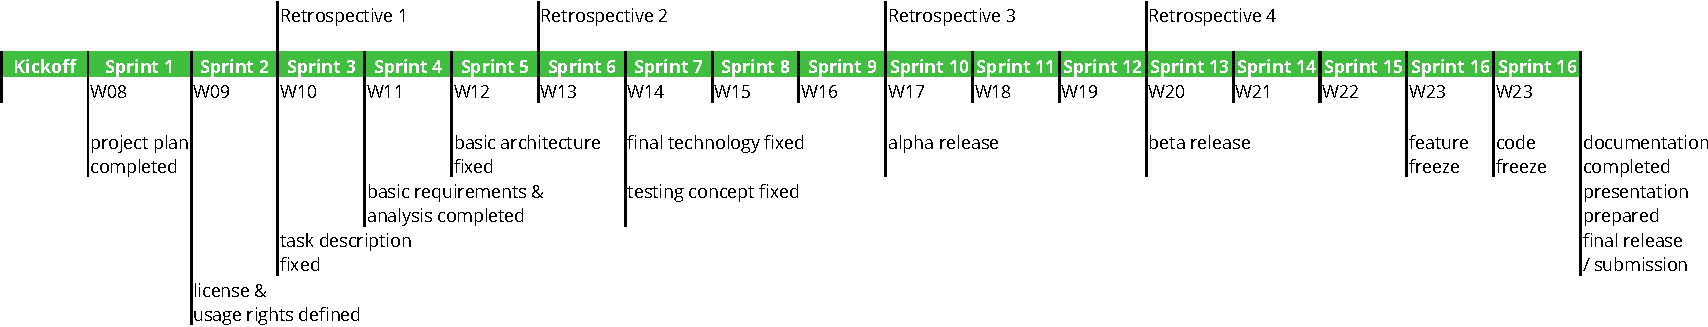
\includegraphics[width=1\linewidth]{resources/overview}
    \caption{Overview of the 16 iterations}
    \label{fig:overview}
\end{figure}

The goals and milestones resulting from each sprint are shown in Figure \ref{fig:sprint-details}.

\begin{figure}[h]
    \begin{sideways}
    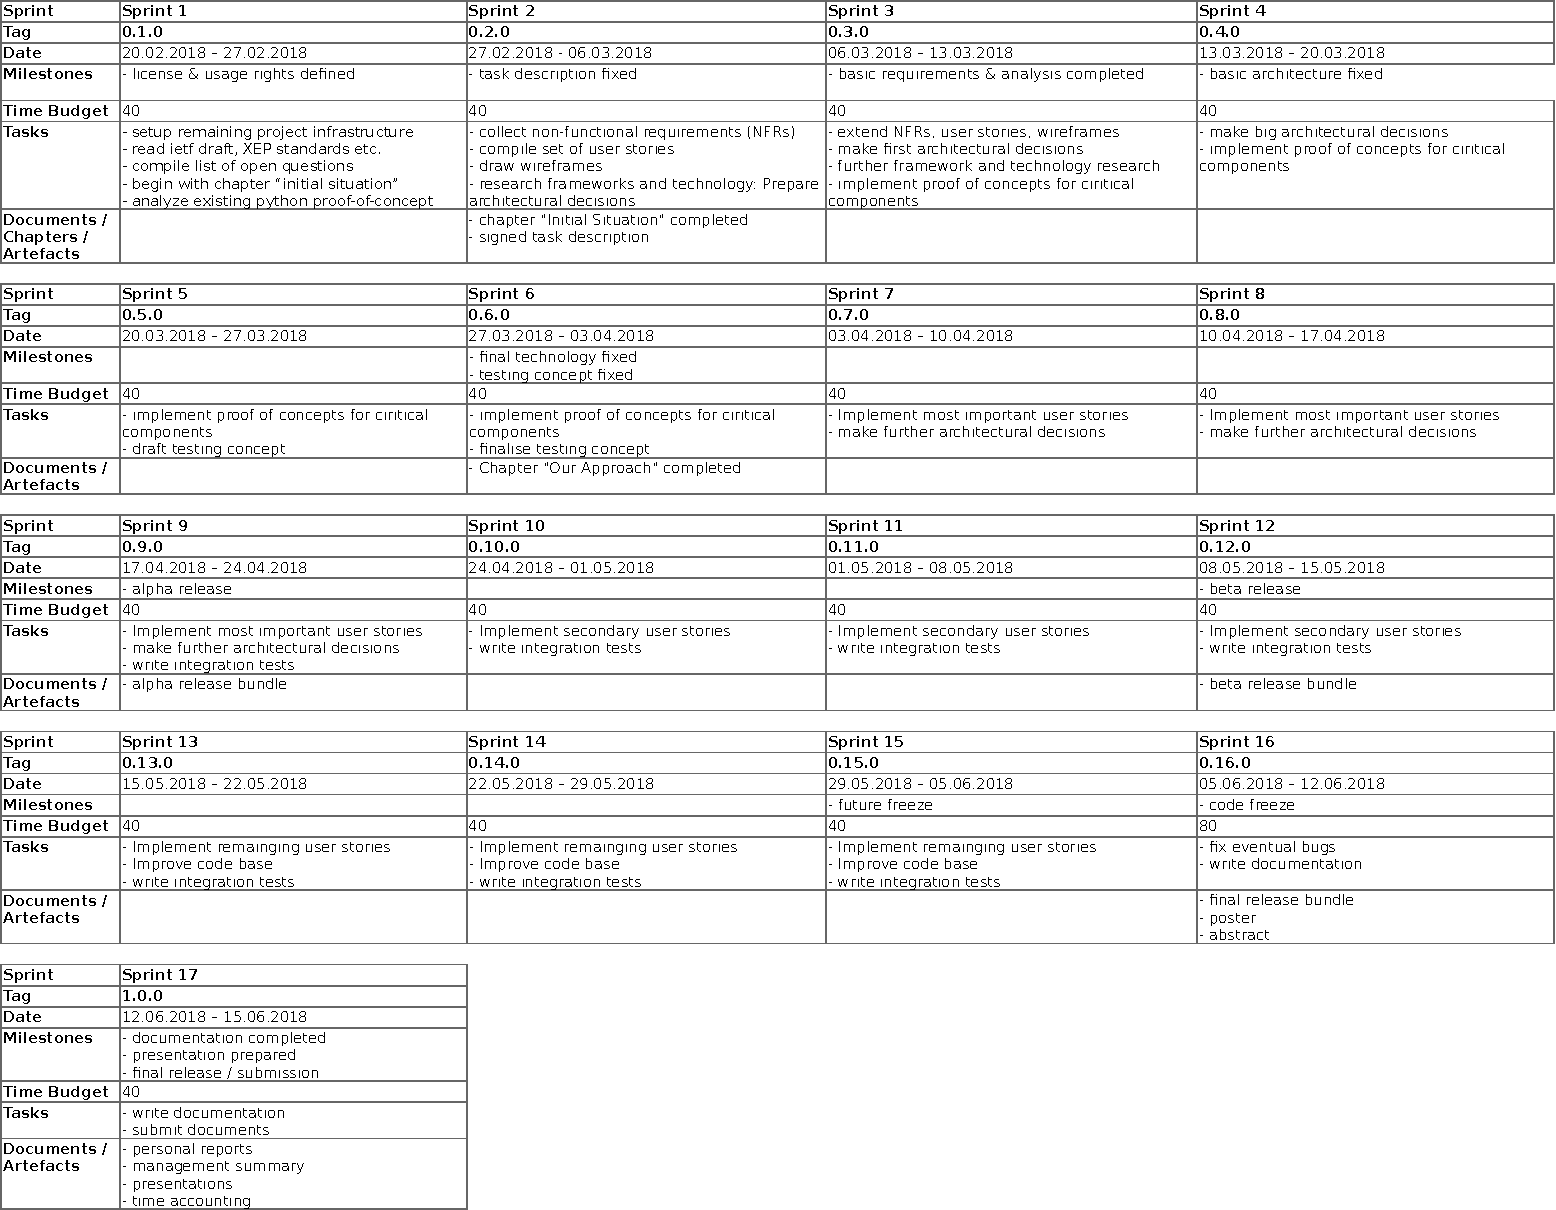
\includegraphics[scale=0.75]{resources/sprint_details}
    \end{sideways}
    \centering
    \caption{Detailed overview with tasks and milestones of all 16 sprints.}
    \label{fig:sprint-details}
\end{figure}


\subsection{Meetings}
The team works every Monday (08:00 - 12:00) and Tuesday (08:00 - 17:00) together in the study room and remotely Fridays (08:00 - 17:00). Wednesday and Friday begin with a daily stand-up meeting taking no longer than 15 minutes. Sprint planning meetings are carried out on Tuesday at 10:00. Table \ref{meeting-time-budget} shows an overview of the total meeting time budget.

\begin{table}[]
    \centering
    \caption{Meeting Time Budget}
    \label{meeting-time-budget}
    \begin{tabular}{lll}
        \hline
        \textbf{Meeting Type}             & \textbf{Total Duration per Person} & \textbf{Total Duration for the Team} \\ \hline
        \textbf{Supervision Meetings}     & 12 hours                           & 24 hours                             \\
        \textbf{Standup Meetings}         & 16 hours                            & 32 hours                             \\
        \textbf{Sprint Planning Meetings} & 18 hours                           & 36 hours                             \\
        \textbf{Retrospective}            & 4 hours                            & 8 hours                              \\ \hline
        \textbf{Total}                    & 50 hours                           & 100 hours
    \end{tabular}
\end{table}

Regular meetings with the project advisor take usually place on Monday in Prof. Dr. Steffen's office.

Raphael Zimmermann will take meeting notes for every meeting. Meeting minutes are published on the project website afterwards.

\chapter{Risk Management}
An assessment of the project-specific risks is carried out in Table \ref{tbl:project-risks} as time loss during the whole project. The risk matrix in Table \ref{tbl:risk-matrix} provides an overview of the risk weighting.

To account for these risks, we reduce our weekly sprint time by the total weighted risk applicable to the planned task topics (on average approximately 13.5\%). We also review the risk assessment after every sprint, adapt it and take measures if necessary.


\begin{table}[h] %TODO: Redefine Risks
    \centering
    \begin{tabu}{|l|c|c|c|}
        \hline
        \diagbox[width=9em,height=2.5em]{Probability}{Severity}
          & High ($\geq 5d$) & Medium (2-5$d$) & Low ($\leq 2d$) \\ \hline
        High ($\geq 60\%$)
          & 1 & & \\ \hline
        Medium (30-60\%)
          & 6 & &  \\ \hline
        Low ($\leq 30\%$)
          & & 3, 4, 5 & \\ \hline
    \end{tabu}
    \caption[Risk matrix]{The risk matrix. Numbers reference to the risk assessment Table \ref{tbl:project-risks}}
    \label{tbl:risk-matrix}
\end{table}


\begin{sidewaystable}
    \centering
    \caption[Risk assessment]{Risk assessment table. Time in hours over the total project duration.}
    \label{tbl:project-risks}
    \begin{tabu}{r l X X r r r}
        \hline
        \# & Title & Description & Prevention / Reaction & Risk [h] & Probability & = [h] \\ \hline

        1 & Incomplete reference documentation
          & The reference documentation / standards are incomplete or difficult to comprehend.
          & Discuss missing parts with project advisor
          & 60 & 60\% & 36\\

        2 & Communication errors
          & Errors due to miscommunication or misapprehension.
          & Maintain a high level of interaction, precise specification of tasks responsibilities, conduct meetings if ambiguities exist.
          & 30 & 50\% & 15\\

        3 & Problems with project infrastructure
          & The used project infrastructure is not or only partially available, or data loss occurs within management software.
          & Clean setup and self-hosting of the tools to prevent third-party dependencies.
          & 45 & 30\% & 13.5 \\

        4 & Scope creep
          & The project's scope is extended over the project course.
          & Define the project scope and limitations precisely. Discuss changes with the project advisor.
          & 45 & 30\% & 13.5\\

        5 & Dependency errors
          & There are errors/bugs in third-party dependencies, i.e. libraries.
          & Carefully select libraries and limit thid-party dependency to a minimum.
          & 30 & 30\% & 9\\

        6 & Missing dependency documentation
          & Selected libraries are lacking proper documentation
          & The documentation quality of a library should be a selection criterion.
          & 30 & 40\% & 12\\

         \hline
        & Total weighted risk & & & & & 99\\
        \hline
    \end{tabu}
\end{sidewaystable}


\chapter{Infrastructure}
\section{Project Management and Development}
For project management we utilise JIRA\cite{atlassian-opensource}. As document/code storage, git repositories on Github are used, the continuous integration/deployment will be defined in the course of the project. %TODO: Add CI/CD tools when defined

These applications are hosted on our HSR project server, which runs a standard Ubuntu Linux 17.10.


\subsection{Development Tools}
The development tools will be defined in the course of the project. %TODO: Add development tools when defined

\section{Backup and Data Safety}
An incremental backup of the project server including the source code and documentation is created on an independent system every night.

As our documents and code is stored in a git repository, they are also distributed on all development systems.


\chapter{Quality Measures}
To maintain a high standard of quality, we take the following measures:

\begin{multicols}{2}
    \begin{itemize}
        \item short sprint reviews
        \item four extended retrospectives
        \item code reviews
        \item automated unit and integration testing
        \item publish all documentation on the project website using continuous integration/delivery.
        \item using continuous integration for source code
    \end{itemize}
\end{multicols}

\section{Documentation}
The official documents such as the final submission document, meeting minutes as well as this project plan are written in \LaTeX~respectively ASCIIDoc and published on the project website \footnote{\url{https://xgb.redbackup.org}} containing all PDF documents.

The sources are in both cases kept under version control in the same repository, which allows us to use the same tools and processes for documentation and code. The continuous integration server builds and publishes the website whenever new changes are pushed to the repository.

\section{Project Management}
Because the project plan allows for an iterative process, we use JIRA with its SCRUM-features (such as sprint creation or boards) for project management.

\subsection{Sprint Planning}
Each sprint is mapped to JIRA, which allows the project advisor to trace the project progress. Sprints are represented as boards on which the current state and assignee of any issue is easily visible ("To Do", "In Progress", "Review", "Done").


\subsection{Definition of Done}
An issue may be closed if \emph{all} of the following conditions are met:

\begin{itemize}
    \item All functionality conforms to the specification. Any deviations must be discussed and decided by the team.
    \item The source code is reasonably documented.
    \item No code is commented out.
    \item No warnings and errors by the compiler or any other quality tool.
    \item A review is performed and accepted in a pull request.
    \item The corresponding branch is merged into the stable branch (e.g. master).
    \item All documents are up to date including the project website.
    \item Reasonable unit and integration tests exist and pass.
    \item The complete continuous integration pipeline works.
    \item All time is logged.
\end{itemize}

\section{Development}

We decided to use GitHub Flow\cite{github-flow}, a straightforward development workflow.

\begin{figure}[H]
    \centering
    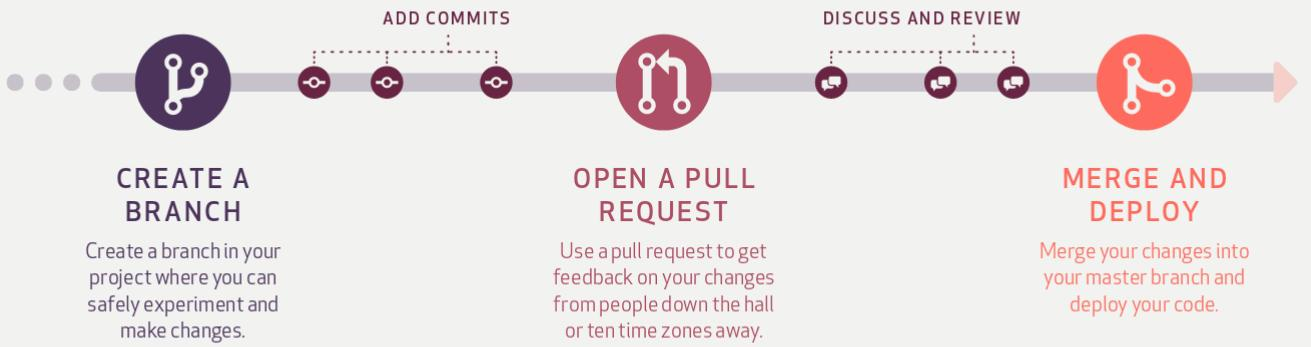
\includegraphics[width=0.85\linewidth]{resources/github_flow}
    \caption[Organigram]{GitHub Flow illustrated ( Source \cite{github-flow})}
    \label{fig:organigram}
\end{figure}


Since the effective technology will be fixed later in the project, concrete coding guidelines, tools, metrics and an error policy will be defined when appropriate.


\section{Testing}
All functionality must be automatically testable using continuous integration. Any non-trivial function/method must be verified with unit tests.

Integration tests verify extended test scenarios.

A minimal performance analysis will be carried out at the end of the project.



\label{lastpage} %TODO: This label should be positioned below above the last paragraph

%\cleardoublepage
%----------------------------------------------------------------------------------------
%    BIBLIOGRAPHY
%----------------------------------------------------------------------------------------
\backmatter
\pagenumbering{Roman}

\bibliographystyle{abbrv}
\bibliography{references}
\addcontentsline{toc}{chapter}{Bibliography}


%----------------------------------------------------------------------------------------
%    LIST OF FIGURES/TABLES PAGES
%----------------------------------------------------------------------------------------

\listoffigures % Prints the list of figures

\listoftables % Prints the list of tables

%----------------------------------------------------------------------------------------
%    ABBREVIATIONS
%----------------------------------------------------------------------------------------

\begin{abbreviations}{ll} % Include a list of abbreviations (a table of two columns)

%\textbf{LAH} & \textbf{L}ist \textbf{A}bbreviations \textbf{H}ere\\
%\textbf{WSF} & \textbf{W}hat (it) \textbf{S}tands \textbf{F}or\\

\end{abbreviations}

\end{document}
